\documentclass[11pt]{article}


%%% Packages
%%
\usepackage{amsmath}
\usepackage{amsfonts}
\usepackage{amssymb}
\usepackage{fancyhdr}
\usepackage{float}
\usepackage{graphicx}
\usepackage{listings}
\usepackage{enumitem}
\usepackage[margin = 1in, headheight = 13.6pt]{geometry}
\usepackage[linktoc=all]{hyperref}
%%
%%%


%%% Formatting
%%
\parindent 0em
\parskip 1em
\pagestyle{fancy}
\fancyhead{}
\fancyfoot{}
\fancyhead[L]{\slshape\MakeUppercase{{\myTitle}}}
\fancyhead[R]{\slshape{\myName}}
\fancyfoot[C]{\thepage}
%%
%%%


%%% User defined variables
%%
\def \myTitle {ECE 302 Homework 1}
\def \myName {Elias Talcott}
\def \myDate {September 4, 2020}
%%
%%%


\begin{document}

\section*{Exercise 9 Code}
\lstinputlisting[language=Python, breaklines=True]{exercise9.py}

\section*{Exercise 9 Result}
\begin{enumerate}[label=(\alph*)]
\item Result: $[14, 32, 50]$
\pagebreak
\item sin(x) on [-$\pi$, $\pi$] for 1000 data points of x
\begin{figure}[h!]
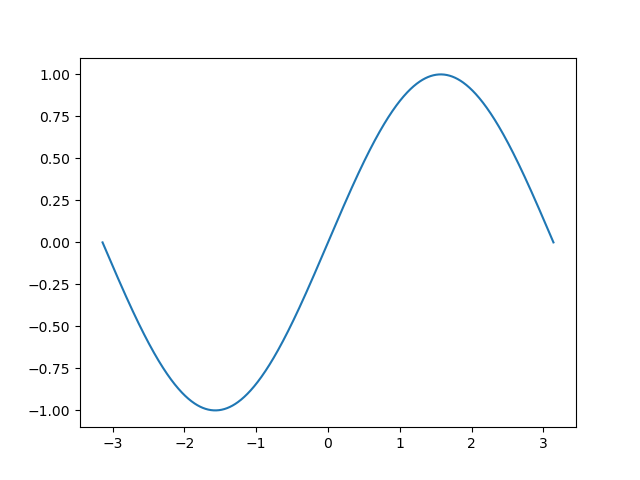
\includegraphics[width=0.7\linewidth]{figure9_b.png}
\end{figure}
\item 10,000 uniformly distributed random numbers on [0, 1)
\begin{figure}[h!]
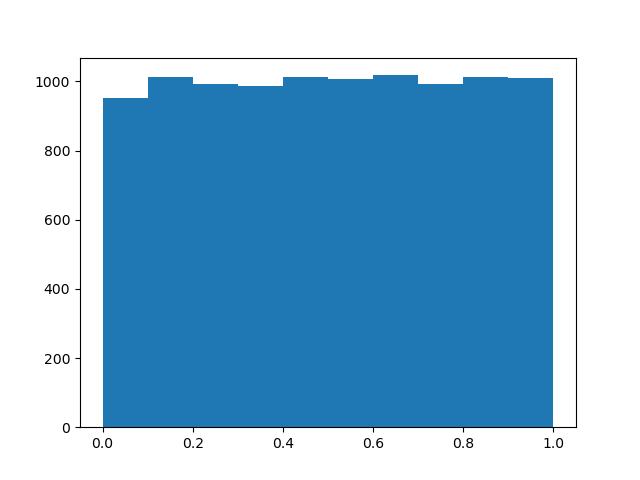
\includegraphics[width=0.7\linewidth]{figure9_c.png}
\end{figure}
\end{enumerate}

\pagebreak

\section*{Exercise 10 Code}
\lstinputlisting[language=Python, breaklines=True]{exercise10.py}

\section*{Exercise 10 Result}
\begin{enumerate}[label=(\alph*)]
\item Fraction of draws with one vowel and one consonant: 0.3366
\end{enumerate}

\pagebreak

\section*{Exercise 11 Code}
\lstinputlisting[language=Python, breaklines=True]{exercise11.py}

\section*{Exercise 11 Result}
\begin{enumerate}[label=(\alph*)]
\item Fraction of simulations with at least one matching birthday: 0.9676
\end{enumerate}

\end{document}